\documentclass{beamer}
\usepackage[utf8]{inputenc}
\usepackage[T1]{fontenc}
\usepackage{setspace}
\usepackage{gensymb}
\singlespacing
\usepackage{amsmath}
\usepackage{amssymb}
\usepackage{bm}
\usepackage{cite}
\usepackage{cases}
\usepackage{subfig}
\usepackage{longtable}
\usepackage{multirow}
\usepackage{verbatim}
\usepackage{hyperref}
\usepackage{listings}
\usepackage{xcolor}
\usepackage{array}
\usepackage{calc}
\usepackage{hhline}
\usepackage{ifthen}
\usepackage{textcomp}
\hypersetup{
    colorlinks=true,
    linkcolor=black,
    urlcolor=blue,
}

\usetheme{CambridgeUS}

% Robust listings configuration
\lstset{
    basicstyle=\ttfamily\footnotesize,
    breaklines=true,
    postbreak={\mbox{\textcolor{red}{\tiny$\hookrightarrow$}\space}},
    columns=fullflexible,
    keepspaces=true,
    showstringspaces=false,
    upquote=true,
    literate={~}{{\textasciitilde}}1
}

\title[Digital Clock Implementation]{Digital Clock Implementation using Arduino with Multiplexing and Editing Features}
\author{Dhawal}
\institute[IITH]{
    Department of Electrical Engineering\\
    Indian Institute of Technology Hyderabad\\
    Email: ee24btech11015@iith.ac.in
}
\date{}

\begin{document}

\begin{frame}
    \titlepage
    \centering
    Electrical Engineering Department\\
    Indian Institute of Technology, Hyderabad
\end{frame}

\begin{frame}{Outline}
    \tableofcontents
\end{frame}

\section{Introduction}
\begin{frame}{Introduction}
    \begin{itemize}
        \item Digital clock system with editing capabilities using Arduino microcontroller
        \item Key features:
        \begin{itemize}
            \item Multiplexing technique for six 7-segment displays
            \item Minimal I/O pin usage
            \item Pause/play functionality
            \item Digit-by-digit editing with increment/decrement buttons
        \end{itemize}
        \item Comprehensive Boolean logic for time constraints
    \end{itemize}
\end{frame}

\section{Components}
\begin{frame}{Components}
    \begin{table}
        \centering
        \begin{tabular}{|l|c|c|}
        \hline
        \textbf{Component} & \textbf{Value} & \textbf{Quantity}\\
        \hline
        Arduino Uno & & 1\\
        \hline
        USB Cable & Type B & 1\\
        \hline
        Seven Segment Display & Common Cathode & 6\\
        \hline
        Push Buttons & & 4\\
        \hline
        IC 7447 & & 1\\
        \hline
        Jumper Wires & M-M & 16\\
        \hline
        Breadboard & & 1\\
        \hline
        Resistors & 220$\Omega$ & 7\\
        \hline
        Resistors & 10$k\Omega$ & 4\\
        \hline
        \end{tabular}
        \caption{Components List}
    \end{table}
\end{frame}

\section{Circuit Connections}
\begin{frame}{Arduino Pin Connections}
    \begin{table}
        \centering
        \begin{tabular}{|c|c|c|}
        \hline
        \textbf{Item} & \textbf{Arduino Pin} & \textbf{Function}\\
        \hline
        Button 1 & A0 (PC0) & Edit Mode Toggle\\
        \hline
        Button 2 & A1 (PC1) & Next Digit Selection\\
        \hline
        Button 3 & A2 (PC2) & Increment Digit\\
        \hline
        Button 4 & A3 (PC3) & Decrement Digit\\
        \hline
        IC 7447 Pin 7 & D2 & BCD Bit 0 (LSB)\\
        \hline
        IC 7447 Pin 1 & D3 & BCD Bit 1\\
        \hline
        IC 7447 Pin 2 & D4 & BCD Bit 2\\
        \hline
        IC 7447 Pin 6 & D5 & BCD Bit 3 (MSB)\\
        \hline
        Display 1 & D6 & Hours Tens Digit\\
        \hline
        Display 2 & D7 & Hours Units Digit\\
        \hline
        Display 3 & D8 & Minutes Tens Digit\\
        \hline
        Display 4 & D9 & Minutes Units Digit\\
        \hline
        Display 5 & D10 & Seconds Tens Digit\\
        \hline
        Display 6 & D11 & Seconds Units Digit\\
        \hline
        \end{tabular}
        \caption{Arduino Pin Connections}
    \end{table}
\end{frame}



\section{Multiplexing Technique}
\begin{frame}{Multiplexing Technique}
    \begin{itemize}
        \item All segment inputs connected to single BCD decoder
        \item Digital pins control common cathode of each display
        \item Selective activation of displays
        \item 2ms time gap between display switching
        \item Creates illusion of simultaneous operation
        \item Minimal I/O pin usage (only 6 pins for displays)
    \end{itemize}
\end{frame}

\section{Digit Editing Logic}
\begin{frame}{Editing System Overview}
    \begin{enumerate}
        \item Button 1: Toggles between run mode and edit mode
        \item Button 2: Cycles through six digits in edit mode
        \item Button 3: Increments selected digit with rollover constraints
        \item Button 4: Decrements selected digit with rollunder constraints
    \end{enumerate}
    
    \vspace{0.5cm}
    Different constraints based on digit position:
    \begin{itemize}
        \item Units digits: 0-9
        \item Tens of minutes/seconds: 0-5
        \item Tens of hours: 0-2
    \end{itemize}
\end{frame}

\begin{frame}{Increment Logic - Units Digits (0-9)}
    \begin{columns}
        \begin{column}{0.5\textwidth}
            \begin{table}
                \centering
                \scriptsize
                \begin{tabular}{|c|c|c|c|c|c|c|c|}
                \hline
                D & C & B & A & $D_1$ & $C_1$ & $B_1$ & $A_1$ \\ 
                \hline
                0 & 0 & 0 & 0 & 0 & 0 & 0 & 1 \\
                0 & 0 & 0 & 1 & 0 & 0 & 1 & 0 \\
                0 & 0 & 1 & 0 & 0 & 0 & 1 & 1 \\
                0 & 0 & 1 & 1 & 0 & 1 & 0 & 0 \\
                0 & 1 & 0 & 0 & 0 & 1 & 0 & 1 \\
                0 & 1 & 0 & 1 & 0 & 1 & 1 & 0 \\
                0 & 1 & 1 & 0 & 0 & 1 & 1 & 1 \\
                0 & 1 & 1 & 1 & 1 & 0 & 0 & 0 \\
                1 & 0 & 0 & 0 & 1 & 0 & 0 & 1 \\
                1 & 0 & 0 & 1 & 0 & 0 & 0 & 0 \\
                \hline
                \end{tabular}
            \end{table}
        \end{column}
        \begin{column}{0.5\textwidth}
            Simplified Boolean expressions:
            \begin{align*}
                A_1 &= A' \\
                B_1 &= A + B \\
                C_1 &= AB + C \\
                D_1 &= ABC + D
            \end{align*}
        \end{column}
    \end{columns}
\end{frame}

\begin{frame}{Increment Logic - Tens of Minutes/Seconds (0-5)}
    \begin{columns}
        \begin{column}{0.5\textwidth}
            \begin{table}
                \centering
                \scriptsize
                \begin{tabular}{|c|c|c|c|c|c|c|c|}
                \hline
                D & C & B & A & $D_1$ & $C_1$ & $B_1$ & $A_1$ \\ 
                \hline
                0 & 0 & 0 & 0 & 0 & 0 & 0 & 1 \\
                0 & 0 & 0 & 1 & 0 & 0 & 1 & 0 \\
                0 & 0 & 1 & 0 & 0 & 0 & 1 & 1 \\
                0 & 0 & 1 & 1 & 0 & 1 & 0 & 0 \\
                0 & 1 & 0 & 0 & 0 & 1 & 0 & 1 \\
                0 & 1 & 0 & 1 & 0 & 0 & 0 & 0 \\
                \hline
                \end{tabular}
            \end{table}
        \end{column}
        \begin{column}{0.5\textwidth}
            Simplified Boolean expressions:
            \begin{align*}
                A_1 &= A'B'C' + AB'C \\
                B_1 &= A'BC' + AB'C' \\
                C_1 &= A'BC + AB'C \\
                D_1 &= 0
            \end{align*}
        \end{column}
    \end{columns}
\end{frame}

\begin{frame}{Increment Logic - Tens of Hours (0-2)}
    \begin{columns}
        \begin{column}{0.5\textwidth}
            \begin{table}
                \centering
                \scriptsize
                \begin{tabular}{|c|c|c|c|c|c|c|c|}
                \hline
                D & C & B & A & $D_1$ & $C_1$ & $B_1$ & $A_1$ \\ 
                \hline
                0 & 0 & 0 & 0 & 0 & 0 & 0 & 1 \\
                0 & 0 & 0 & 1 & 0 & 0 & 1 & 0 \\
                0 & 0 & 1 & 0 & 0 & 0 & 0 & 0 \\
                \hline
                \end{tabular}
            \end{table}
        \end{column}
        \begin{column}{0.5\textwidth}
            Simplified Boolean expressions:
            \begin{align*}
                A_1 &= A'B' \\
                B_1 &= AB' \\
                C_1 &= 0 \\
                D_1 &= 0
            \end{align*}
        \end{column}
    \end{columns}
\end{frame}

\begin{frame}{Decrement Logic - Units Digits (0-9)}
    \begin{columns}
        \begin{column}{0.5\textwidth}
            \begin{table}
                \centering
                \scriptsize
                \begin{tabular}{|c|c|c|c|c|c|c|c|}
                \hline
                D & C & B & A & $D_1$ & $C_1$ & $B_1$ & $A_1$ \\ 
                \hline
                0 & 0 & 0 & 0 & 1 & 0 & 0 & 1 \\
                0 & 0 & 0 & 1 & 0 & 0 & 0 & 0 \\
                0 & 0 & 1 & 0 & 0 & 0 & 0 & 1 \\
                0 & 0 & 1 & 1 & 0 & 0 & 1 & 0 \\
                0 & 1 & 0 & 0 & 0 & 0 & 1 & 1 \\
                0 & 1 & 0 & 1 & 0 & 1 & 0 & 0 \\
                0 & 1 & 1 & 0 & 0 & 1 & 0 & 1 \\
                0 & 1 & 1 & 1 & 0 & 1 & 1 & 0 \\
                1 & 0 & 0 & 0 & 0 & 1 & 1 & 1 \\
                1 & 0 & 0 & 1 & 1 & 0 & 0 & 0 \\
                \hline
                \end{tabular}
            \end{table}
        \end{column}
        \begin{column}{0.5\textwidth}
            Simplified Boolean expressions:
            \begin{align*}
                A_1 &= A \\
                B_1 &= A' + B \\
                C_1 &= A'B' + C \\
                D_1 &= A'B'C' + D
            \end{align*}
        \end{column}
    \end{columns}
\end{frame}

\begin{frame}{Decrement Logic - Tens of Minutes/Seconds (0-5)}
    \begin{columns}
        \begin{column}{0.5\textwidth}
            \begin{table}
                \centering
                \scriptsize
                \begin{tabular}{|c|c|c|c|c|c|c|c|}
                \hline
                D & C & B & A & $D_1$ & $C_1$ & $B_1$ & $A_1$ \\ 
                \hline
                0 & 0 & 0 & 0 & 0 & 1 & 0 & 1 \\
                0 & 0 & 0 & 1 & 0 & 0 & 0 & 0 \\
                0 & 0 & 1 & 0 & 0 & 0 & 0 & 1 \\
                0 & 0 & 1 & 3 & 0 & 0 & 1 & 0 \\
                0 & 1 & 0 & 0 & 0 & 0 & 1 & 1 \\
                0 & 1 & 0 & 1 & 0 & 1 & 0 & 0 \\
                \hline
                \end{tabular}
            \end{table}
        \end{column}
        \begin{column}{0.5\textwidth}
            Simplified Boolean expressions:
            \begin{align*}
                A_1 &= A'B'C + AB'C' \\
                B_1 &= A'BC' + AB'C' \\
                C_1 &= A'B'C' + ABC' \\
                D_1 &= 0
            \end{align*}
        \end{column}
    \end{columns}
\end{frame}

\begin{frame}{Decrement Logic - Tens of Hours (0-2)}
    \begin{columns}
        \begin{column}{0.5\textwidth}
            \begin{table}
                \centering
                \scriptsize
                \begin{tabular}{|c|c|c|c|c|c|c|c|}
                \hline
                D & C & B & A & $D_1$ & $C_1$ & $B_1$ & $A_1$ \\ 
                \hline
                0 & 0 & 0 & 0 & 0 & 0 & 1 & 0 \\
                0 & 0 & 0 & 1 & 0 & 0 & 0 & 0 \\
                0 & 0 & 1 & 0 & 0 & 0 & 0 & 1 \\
                \hline
                \end{tabular}
            \end{table}
        \end{column}
        \begin{column}{0.5\textwidth}
            Simplified Boolean expressions:
            \begin{align*}
                A_1 &= BA' \\
                B_1 &= B'A' \\
                C_1 &= 0 \\
                D_1 &= 0
            \end{align*}
        \end{column}
    \end{columns}
\end{frame}


\begin{frame}{Hardware Build}
    \begin{columns}
        \begin{column}{0.6\textwidth}
            \begin{itemize}
                \item Connect seven-segment displays to breadboard
                \item Connect all segment outputs together (through resistors)
                \item Make connections to IC7447
                \item Connect IC7447 and buttons to Arduino
                \item Add current-limiting resistors for LEDs
                \item Add pull-down resistors for buttons
            \end{itemize}
        \end{column}
        \begin{column}{0.4\textwidth}
            \centering
            \includegraphics[width=0.9\textwidth]{figs/clock.jpg}
            \scriptsize Final Arduino-based Clock Implementation
        \end{column}
    \end{columns}
\end{frame}

\begin{frame}{Tinkercad Simulation}
    \centering
    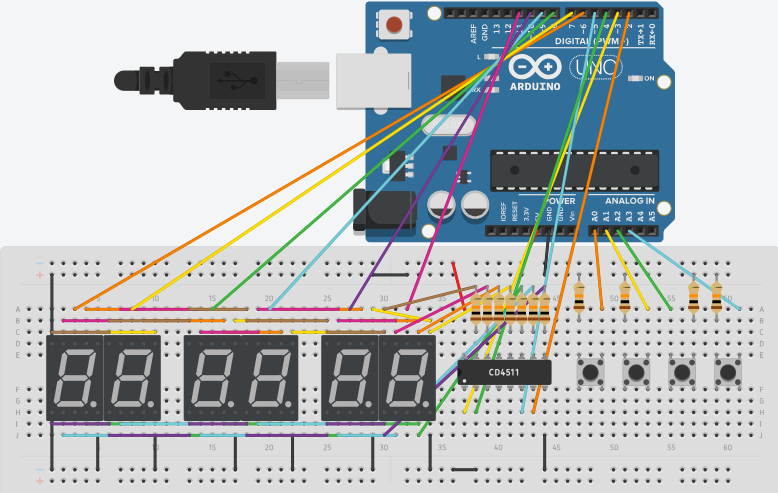
\includegraphics[width=0.7\textwidth]{figs/Clock_Tinkercad.png}
    \scriptsize Tinkercad Simulation of the Digital Clock
\end{frame}

\section{Conclusion}
\begin{frame}{Summary}
    \begin{itemize}
        \item Successfully implemented digital clock with editing features
        \item Key achievements:
        \begin{itemize}
            \item Efficient multiplexing technique
            \item Comprehensive editing system
            \item Boolean logic implementation
            \item Minimal I/O pin usage
        \end{itemize}
        \item Complete documentation and source code available
    \end{itemize}
\end{frame}

\begin{frame}{Acknowledgment}
    \centering
    \Large
    The complete source code and documentation can be found at:\\
    \vspace{0.5cm}
    \url{https://github.com/Dhawal24112006/projects.git}
    
    \vspace{1cm}
    \normalsize
    Thank You!
\end{frame}



\end{document}
